\documentclass[oneside]{book}
\usepackage[utf8]{inputenc}
\usepackage{fancyhdr}
\usepackage{listings}
\usepackage[document]{ragged2e}
\usepackage{lastpage}
\usepackage{circuitikz}
\usepackage{amsmath}
\usepackage{amssymb}
\usepackage{mathrsfs, amsmath}
\usepackage{amsfonts}
\usepackage{amsthm}
\usepackage{caption}
\usepackage{subcaption}
\usepackage{tcolorbox}
\usepackage{cancel}
\usepackage{nccmath}
\usepackage{wrapfig}
\usepackage{hyperref,lipsum}
\usepackage[export]{adjustbox}
%\usepackage{fullpage}
\usepackage{geometry}
\usepackage{listings}
\usepackage{textcomp}
\pagestyle{fancy}
\fancyhf{}
\fancyhead[L]{\leftmark} % Chapter name at the left header
\fancyhead[R]{\thepage} % Page number at the right header
\renewcommand{\chaptermark}[1]{\markboth{#1}{}}
\hypersetup{
    colorlinks=true,
    linkcolor=blue,
    filecolor=magenta,      
    urlcolor=cyan,
    pdftitle={Overleaf Example},
    pdfpagemode=FullScreen,
    }
\begin{document}
\begin{titlepage}
\centering
{\bfseries\Huge Indian Institute of Technology Hyderabad\par}


\vfill
\noindent
{\bfseries\Huge SciTech Project  \par}
\bigskip%Título
\vspace{0.5cm}

{\bfseries\scshape Odometry and motion tracking \par}
\vspace{0.5cm}
\noindent
\vfill
{\Large K Rahul\par}
{\Large ee23btech11027 \par}
\vfill
\end{titlepage}
\setcounter{page}{0}


\newpage
\tableofcontents
\newpage
\Large

\chapter{Introduction} \label{Chapter-1}
This project attemps to collect accelerometer data from a sensor, sampled at some time, and give an output about the displacement of the object. An advancement of using a Kalman Filter to filter out any noise from the sensor has also been undertaken.\\ 
This document describes the implementation of the aforementioned. \\
\bigskip
The data has been collected using an android app named Phyphox. This app uses the sensors present in the phone to continously keep track of the acceleration of the phone. After the collection of the data, after moving around with the phone, the sensor data is then input into a CSV file. This CSV file contains the value of acceleration in the $x$, $y$ and $z$ directions(as well as the magnitude, but that is largely not useful for the purposes of tracking motion) sampled at some time intervals. The important thing to note is that this sampling interval is not regular, although generally, the sampling intervals differ only by an order of $10^{-4}$ seconds. 

\newpage
\chapter{Calculation of displacement from acceleration}
Acceleration is recorded as discrete data points sampled at some time $t$. This begs the question - How do we find the position of the object from acceleration? The first option that comes to mind is just to integrate the acceleration twice w.r.t time in order to obtain displacement.\\
\bigskip
There exist potent ways of calculating an integral using a computer, one of which would be using trapezoidal integration. Given a function $y = f(x)$, an arbitrarily small trapezoidal height, say $\epsilon$ can be fixed(so points taken would be $x$ and $x + \epsilon$, for some $x$ in the domain of $f(x)$), and the length of the parallel sides would be $f(x)$ and $f(x+\epsilon)$,using which we find the area of the extremely small trapezium and sum the areas of the previous small trapeziums in order to find out the value of the integral. Doing this twice \textit{should}, in theory, give us the displacement.\\
\bigskip
However, upon carrying out this exercise, it gave disappointingly bad results. If that was not bad, doing trapezoidal integration twice ended up giving the same kind of curve, no matter what experiment was done (i.e, even if the data for acceleration from two different experiments were wildly different, trapezoidal integration done twice ended up giving the exact same curve structure). This cannot be any good, so one has to turn to other ways to calculate the integral.\\
\bigskip 
The Fourier transform turns out to be a surprisingly reliable way to carry out such integration. The illustration of how to go about it is as follows.\\
\begin{enumerate}
    \item $a(t)$ and $A(f)$ correspond to acceleration in time and frequency domain respectively.
    \item $v(t)$ and $V(f)$ correspond to velocity in time and frequency domain respectively.
    \item $x(t)$ and $X(f)$ correspond to position in time and frequency domain respectively
\end{enumerate}
\begin{align}
    a(t) &= \int_{-\infty}^{+\infty} A(f)e^{j2\pi ft} df \label{FT_acc} \\
    v(t) &= \int_{-\infty}^{+\infty} V(f)e^{j2\pi ft} df \label{FT_vel}\\
    x(t) &= \int_{-\infty}^{+\infty} X(f)e^{j2\pi ft} df \label{FT_pos}
\end{align}
Taking derivative w.r.t $t$ of \eqref{FT_vel} once and \eqref{FT_pos} twice, and comparing with \eqref{FT_acc},
\begin{align}
    A(f) &= j2 \pi f  V(f)\\
    &= -4 \pi^2 f^2  X(f)
\end{align}
Thus, to obtain velocity, the Fourier transform of acceleration can be divided by frequency, and it's inverse Fourier transform obtains velocity, and this exercise can be repeated with velocity to obtain position.(An interesting observation from this would be that differentiation would act like a high-pass filter and integration would act be a low-pass filter, albeit probably not that useful of a filter.)\\
\newpage
\chapter{Using the Fourier Transform on the discrete data set}
While the above reasoning is correct, it only applies in the continuous domain. However, the sensor provides discrete data, so it cannot be applied directly. One way to go around this problem is to simply sample the signal in frequency domain at a suitably chosen sampling frequency $f_s$(the details of choosing such $f_s$ would be discussed later). \\
Sampling the continuous Fourier Transform at some sampling frequency yields the Discrete Fourier Transform(DFT). Hence, the job becomes much easier: An FFT can be applied onto the data-set, divided by the sampling frequency(and a suitable scaling factor), and it's IFFT computed to find the integral. But an N-point DFT requires that all points be sampled regularly(i.e, the sampling interval for every measurement must be equal), which is not so(as stated in the \autoref{Chapter-1}).

\chapter{Interpolation}
(The details about filtering the data before interpolation would be clarified later.)\\
Let the values of a function $y = f(x)$ be given at certain points, say $\Bigl(x_i,f\left(x_i\right)\Bigr)$, $\Bigl(x_{i+1}, f(x_{i+1})\Bigr)$, and the task to find the value of the function at $x_i + \epsilon$, i.e,\\ $f(x_i + \epsilon)$, where $0<\epsilon < (x_{i+1} - x_i)$, is assigned. This task would be carried out using interpolation. \\
\bigskip
The simplest way of interpolation would be using linear interpolation(which is what is implemented in the code), wherein an equation of the line connecting the points $\Bigl(x_i,f\left(x_i\right)\Bigr)$ and $\Bigl(x_{i+1}, f(x_{i+1})\Bigr)$ is found, and the value of $f(x_i + \epsilon)$ is found from that so-formed line equation.\\
\bigskip
The code for linear interpolation can be found \href{https://github.com/HarryNyquist/Odometry/blob/main/Codes/2_DataFunctions.cpp}{\underline{\textbf{here}}}, under the function named \verb|linear_interpolation|.\\
\bigskip
The appropriate sampling time $T_s$ is found by taking the minimum time interval of recording of the accelerations (from the Phyphox app as talked about before) and halved. That is,
\begin{align}
    T_s = \frac{\Delta T_{min}}{2}
\end{align}
(It is halved in order to conform to the Nyquist sampling rate, $f_s \geq 2f_{max}$). \\
The code for finding the appropriate sampling rate is found \href{https://github.com/HarryNyquist/Odometry/blob/main/Codes/2_DataFunctions.cpp}{\underline{\textbf{here}}}, under the function named \verb|SamplingTime| \\
\bigskip
Let us say that the first time instant at which the acceleration started getting recorded is from some time $t$(generally, $t \sim 0.02s$), but the interpolation unnecessarily also fills value between 0 and $t$. Hence, to remove the same, the index of the element in the \verb|t| array(it stores the time instants of recording) that is nearest and greater than $t$ is found using the \verb|nearest_index| function, and the array is trimmed using the \verb|trim_time_array| function. \\
\bigskip
Hence, there now exists a new time array, with entries of the form $nT_s$, where $n \in \mathbb{Z}^+$, and new arrays for acceleration in $x$, $y$ and $z$, with their respective values at $nT_s$ found using linear interpolation. These actions are undertaken by the function \verb|uniform_samples|. \\
\chapter{Kalman Filtering} \label{Kalman Filter chapter}
Now to address the elephant in the room - filtering. Filtering is the process by which noise is removed from a system. There are a wide variety of filtering techniques available, and yet choosing them is a task in and of itself. There is no one-size-fits-all filtering technique, hence finding out the right filtering technique is important.\\ 
\bigskip
Now before talking about why Kalman filtering is probably the best way to go, one needs to try other filters to see why they would fail. Let's take the good old Simple Moving Average filter, for example. \\
The reason for why that would not work is that a moving average filter would fail in the presence of rapid extreme variations (which is almost always the case), and averaging them would be a bad idea as they might not account for these extremities properly.
But what if we \textit{did} implement it? Well, it has been, \href{https://github.com/HarryNyquist/Odometry/blob/main/Odometry_Bad_Tries/Bad_Filter_attempts.py}{\underline{\textbf{here}}}, under the function name \verb|simple_moving_average|, after choosing an appropriate \\ \verb|kernel_size|\footnote{if \texttt{kernel\textunderscore size} were to take smaller values, say 10, then it would absolutely follow the output, but offers no amount of filtering whatsoever.It would be equivalent to simply just using the unfiltered output.}. The filtering yielded the following:
\begin{figure}[htbp]
    \centering
    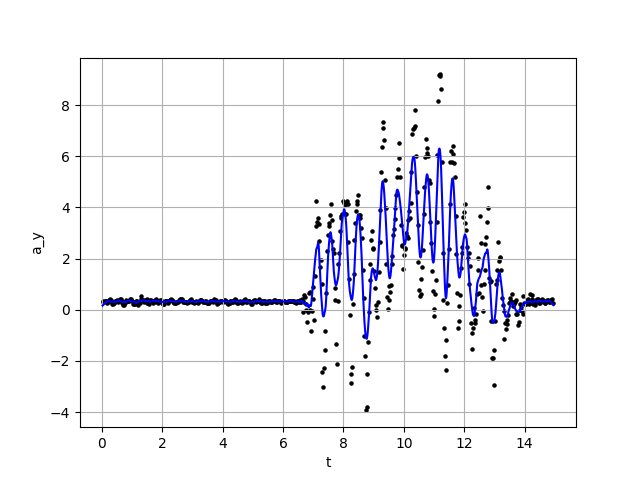
\includegraphics[width=0.8\textwidth]{figs/Filtered_using_SMA_downsampled.png}
    \caption{Filtered vs Original - SMA}
\end{figure}

The black scatter dots represent the actual values, and the blue line represents the filtered values. As it can be seen, the extreme values have not been taken care of properly.  \\
\bigskip
Another option would be to use a Low Pass Filter(LPF). Since we are using a program, a brickwall LPF can be applied onto the signal. (We would have to use a Hamming window function because the brickwall LPF is an IIR filter). This again would be an issue as the cutoff frequency to be set would vary from dataset to dataset. Thus, a cutoff frequency that works for one case might not work for the other. But again, what if it \textit{were} to be implemented?\\
It has been, \href{https://github.com/HarryNyquist/Odometry/blob/main/Odometry_Bad_Tries/Bad_Filter_attempts.py}{\underline{\textbf{here}}}, under the function name \verb|Brickwall_LPF| \footnote{Simply taking the FFT, removing all frequencies above the cutoff, and then taking the IFFT would not always work(in fact, it might not even work for the majority of cases) as the IFFT would return complex values due to lack of conjugate symmetry.}. The filtering yielded the following:
\begin{figure}[htbp]
    \centering
    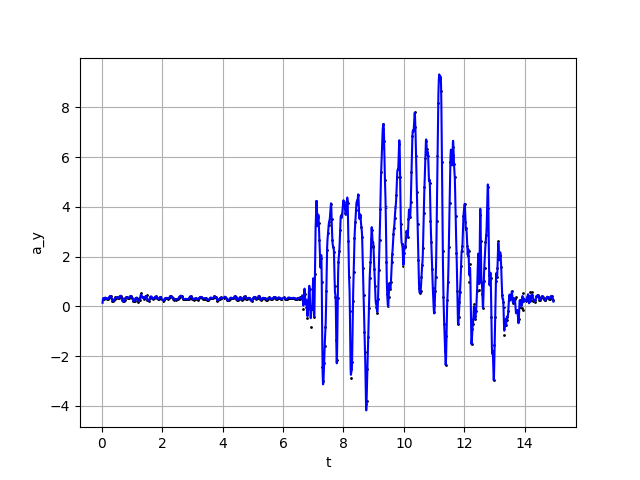
\includegraphics[width=0.8\textwidth]{figs/Filtered_using_brickwall_LPF.png}
    \caption{Filtered vs Original - LPF}
\end{figure}
It would be hard to see it here, but there exists a sort of lag, wherein the filtered output rises (or falls) after the rise (or fall) of the original output. This is not very clear as there are quite a lot of rises and falls, but in data points where there are not too many rises and falls, this would be easier to spot. Nevertheless, the brickwall LPF seems to be a bad idea for this exercise.\\
\bigskip
The common denominator seen is the issue that a particular choice of a filter parameter(for eg., \verb|kernel_size| for the SMA or \verb|cutoff_freq| for the LPF), while working well for one set of data, might not work for another set of data for the same filter parameter used again. Thus, there exists a need for an algorithm that can smartly find out the required filter parameters based on the need. This void is filled by the Kalman Filter(KF).\\ 
\bigskip
Without going too much into the details, the Kalman Filter \footnote{Do note that there are variants of the KF used in modern times, like the EKF, unscented KF etc., which are more accurate but harder to implement.The KF implemented in the code is the original simple KF proposed by Rudolf E. Kálmán} is a recursive algorithm that essentially is given an approximate\\ model \footnote{The approximate model used here assumes that the body undergoes motion with constant jerk, which is correct if taken piecewise. This approximation is surprisingly correct for quite a large portion of the dataset. It only is incorrect at very less number of points, which can be seen upon plotting the acceleration data itself.} that an object would follow, and sensor data about the aforementioned object. The Kalman Filter essentially calculated the Kalman Gain at each recursive step, which in essence, tries to figure out whether to assign a greater weight to the prediction of the model or sensor data based on previous sensor data and model predictions. \\ \bigskip
The code for the Kalman Filter has been implemented \href{https://github.com/HarryNyquist/Odometry/blob/main/Codes/1_KalmanFilter.cpp}{\underline{\textbf{here}}}. A \\ \verb|KalmanFilter| class has been created, with all necessary \\ parameters \footnote{Generally, the parameters for the KF \textit{should} be matrices, but the code has been written as using 1\texttimes 1 matrix, essentially numbers, to make implementation and computation simpler.} required for its operation. Do note that the parameter \verb|R| in the \verb|KalmanFilter| class is initialized to \verb|acc_error|, which is specific to the sensor and can be found beforehand. It has been found to be 0.01 for the sensor on the phone. \newpage
\chapter{Instruction to use}
The most important question as of yet, how is it supposed to be used? The \href{https://github.com/HarryNyquist/Odometry}{\underline{\textbf{GitHub repository}}}, under the directory \verb|Codes|, contain the C++ and Python programs to be run. In \href{https://github.com/HarryNyquist/Odometry/blob/main/Codes/1_KalmanFilter.cpp}{\underline{\textbf{this C++ file}}}, in the following line
\begin{lstlisting}{language=C++}
    ifstream file("May_26_09-16.csv");
\end{lstlisting}
Replace that csv file name with the user's csv file generated by Phyphox(or any other such measurements in csv form) from the user's device.\\
After that, execute the files in order(numbering is given in the file names to indicate the order of execution of the files). 

\chapter{Details about the codes}
The filtering and computation part is done in the directory named \verb|Codes|. The link to the aforementioned directory is \\ \href{https://github.com/HarryNyquist/Odometry/tree/main/Codes}{\underline{\textbf{https://github.com/HarryNyquist/Odometry/tree/main/Codes}}}.\\
\bigskip
\section{Kalman Filtering}
The first file to be run is the following C++ file, for \href{https://github.com/HarryNyquist/Odometry/blob/main/Codes/1_KalmanFilter.cpp}{\textbf{\underline{Kalman Filtering}}}. A \verb|Kalman Filter| class is created first, with the required parameters. \verb|R|, the measurement noise covariance, is specific to the sensor, and has been initialized to the sensor's value in the author's phone. The process noise covariance matrix, \verb|Q|, is generally hard to set, and usually done with some fair amount of trial and error. However, certain general guidelines from previous engineers working on the KF exist, and they make the trial and error process simpler. As with a Kalman Filter, it initially carries out a prediction step via the member function \verb|prediction|, after which it carries out the update step via the member function \verb|update|. The values obtained after Filtering has been written onto a CSV file.

\section{Interpolation}
The second file to be run is the following C++ file, for \href{https://github.com/HarryNyquist/Odometry/blob/main/Codes/2_DataFunctions.cpp}{\textbf{\underline{interpolation}}}. Linear interpolation is carried out using the \verb|linear_interpolation|. Initially, the filtered output from the CSV file from the previous C++ file is read, and then written into vectors. The sampling time initially is found using the Nyquist criterion via the \verb|SamplingTime|, which is then fed to the \verb|linear_interpolation| function along with the original signal to output the linearly interpolated signal at integral multiples of the sampling time. These are again written onto a CSV file. \\
\bigskip
\section{Finding position from acceleration}
The third and final file to be run is the following Python file, for \\
\href{https://github.com/HarryNyquist/Odometry/blob/main/Codes/3_Data_analysis.py}{\textbf{\underline{finding position}}}. The linearly interpolated signal is then read from the CSV file, and written into numpy arrays. Then, as stated earlier, an FFT is taken, suitable manipulations carried out, and IFFT taken to obtain the final position. These values are then written into a CSV file(only for verification though) and the positions in $x$, $y$ and $z$ directions as a function of time $t$ are plotted using Matplotlib.\\
\bigskip
\section{Why not other filters?}
While the Kalman Filtering has given results, an understanding of why other filters are bad choices is crucial in appreciating the value of the KF algorithm. Hence, the following Python file, showcasing \href{https://github.com/HarryNyquist/Odometry/blob/main/Odometry_Bad_Tries/Bad_Filter_attempts.py}{\textbf{\underline{bad filtering attempts}}} is written, and the same data must be used for comparison. \\
\subsection{Simple Moving Average}
A Simple Moving Average filter has been implemented in the aforementioned Python file, using the function \verb|simple_moving_average|. It implements the filter by means of convolution with a kernel of some appropriate size \verb|window_size|. The reasons for abandoning the SMA filter has already been explained in \autoref{Kalman Filter chapter}.\\

\subsection{Low Pass Filter}
A brickwall LPF has been implemented in the aforementioned Python file, using the function \verb|Brickwall_LPF|. A suitable \verb|cutoff_freq|, the cutoff frequency must be chosen. The parameter \verb|num_taps| refers to the number of taps, or the order of the polynomial for performing the Hamming window. The reason for using a Hamming window, and for abandoning the LPF filter, has also been explained in \autoref{Kalman Filter chapter}. 
\end{document}
